\section{Введение}
В данной работе исследуются процессы, протекающие в биполярном транзисторе, с целью экспериментального определения фундаментальной физической константы — отношения заряда электрона к постоянной Больцмана ($e/k$).

\subsection{Цель работы}
\begin{enumerate}
    \item Измерить зависимость тока короткого замыкания коллектора биполярного транзистора от напряжения между эмиттером и базой ($U_{эб}$).
    \item Провести статистическую обработку полученных данных объективным методом парных точек.
    \item По результатам аппроксимации определить величину $e/k$ и сравнить ее с теоретическим значением.
\end{enumerate}

\subsection{Решаемые задачи}
\begin{enumerate}
    \item Собрать измерительную электрическую цепь с биполярным транзистором по схеме с общей базой.
    \item Измерить зависимость $I_k(U_{эб})$ с использованием грубой и точной шкал вольтметра.
    \item Написать программу на языке Python для линейной аппроксимации экспериментальных данных методом парных точек (без использования сторонних статистических библиотек).
    \item Построить экспоненциальные и логарифмические вольт-амперные характеристики (ВАХ).
\end{enumerate}

\section{Основная часть}

\subsection{Теоретическая часть}
При подаче прямого смещения на эмиттерный p-n переход (и коротком замыкании коллекторного), ток коллектора определяется инжекцией неосновных носителей заряда в базу и их последующей диффузией к коллектору. Теоретическая зависимость тока коллектора $I_k$ от напряжения эмиттер-база $U_{эб}$ имеет вид:
\begin{equation}
    I_k = I_0 \left( e^{\frac{e}{kT} U_{эб}} - 1 \right)
\end{equation}
где $I_0$ — тепловой ток насыщения, $T$ — абсолютная температура, $e$ — заряд электрона, $k$ — постоянная Больцмана.

При напряжениях $U_{эб} > 0.1$ В единицей в скобках можно пренебречь. Логарифмируя уравнение, получаем линейную зависимость:
\begin{equation}
    \ln I_k = \ln I_0 + \frac{e}{kT} U_{эб}
    \label{eq:linear}
\end{equation}

Уравнение (\ref{eq:linear}) имеет вид $y = a x + b$, где угловой коэффициент $a = \frac{e}{kT}$. Для нахождения параметров $a$ и $b$ в работе используется объективный \textbf{метод парных точек}. Вектор экспериментальных данных разбивается на две половины, и угловой коэффициент вычисляется усреднением наклонов между соответствующими парами точек:
\begin{equation}
    a_i = \frac{y_{i+N/2} - y_i}{x_{i+N/2} - x_i}, \quad a = \bar{a} = \frac{2}{N} \sum_{i=1}^{N/2} a_i
\end{equation}
Свободный член определяется как $b = \bar{y} - a \bar{x}$. Искомое отношение находится по формуле:
\begin{equation}
    \frac{e}{k} = a \cdot T
\end{equation}
Погрешность косвенного измерения вычисляется по формуле переноса ошибок:
\begin{equation}
    \Delta\left(\frac{e}{k}\right) = \frac{e}{k} \sqrt{\left(\frac{\Delta a}{a}\right)^2 + \left(\frac{\Delta T}{T}\right)^2}
\end{equation}

Размерность искомой величины $e/k$ определяется исходя из рабочей формулы:
\begin{equation*}
    [e/k] =[T \cdot \text{tg}\alpha] = \text{К} \cdot \text{В}^{-1} = \text{К/В}
\end{equation*}

\subsection{Экспериментальная установка}
Для проведения измерений была собрана цепь, в которой транзистор включен по схеме с общей базой (рис. \ref{fig:setup}а). Напряжение $U_{эб}$ регулируется потенциометром и измеряется вольтметром V1. Ток коллектора измеряется косвенно — по падению напряжения на известном резисторе $R_3 = 12$ Ом с помощью вольтметра V2 ($I_k = U_{кб}/R_3$). Сопротивление $R_3$ выбрано достаточно малым, чтобы цепь коллектора можно было считать короткозамкнутой. Внешний вид рабочего стенда представлен на рис. \ref{fig:setup}б.

\begin{figure}[ht!]
    \centering
    \begin{minipage}{0.48\textwidth}
        \centering
        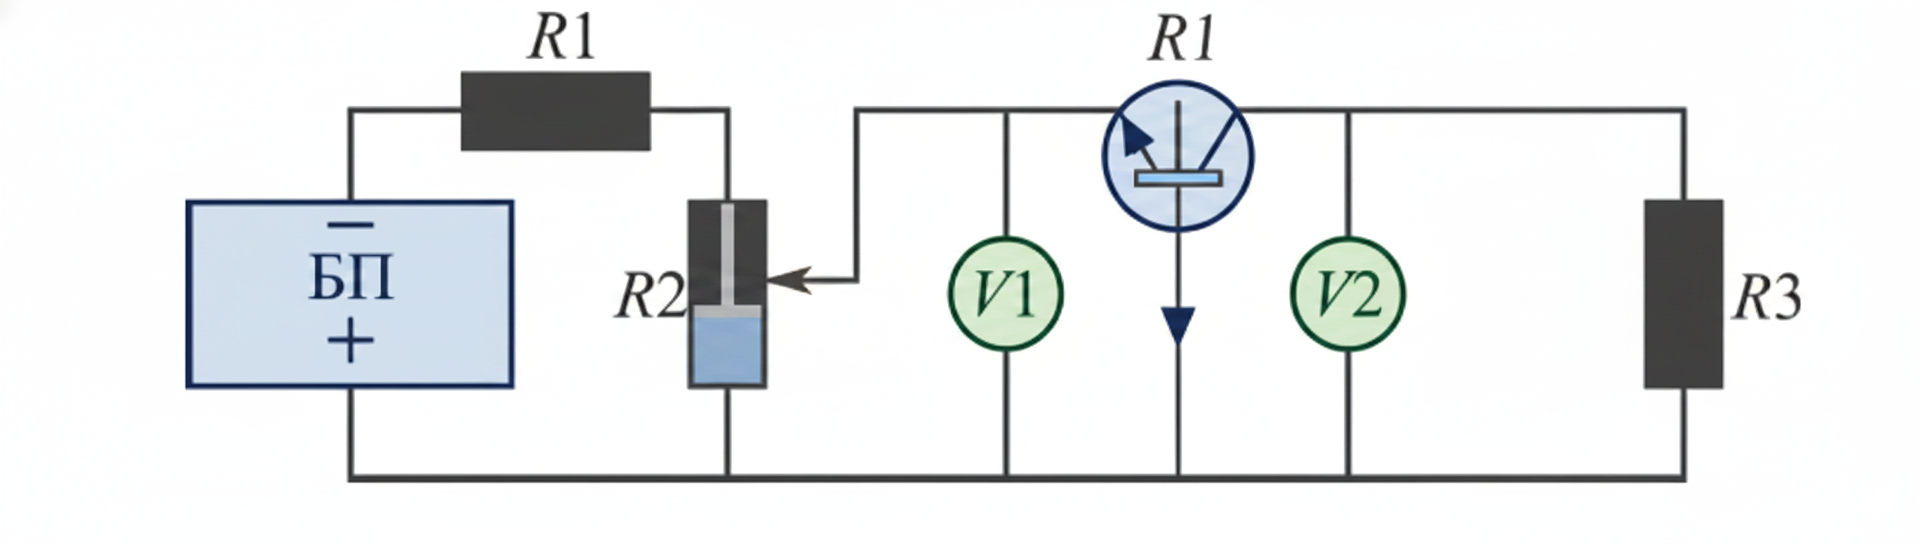
\includegraphics[width=\linewidth]{scheme.png}
        \caption*{а) Принципиальная электрическая схема}
    \end{minipage}
    \hfill
    \begin{minipage}{0.48\textwidth}
        \centering
        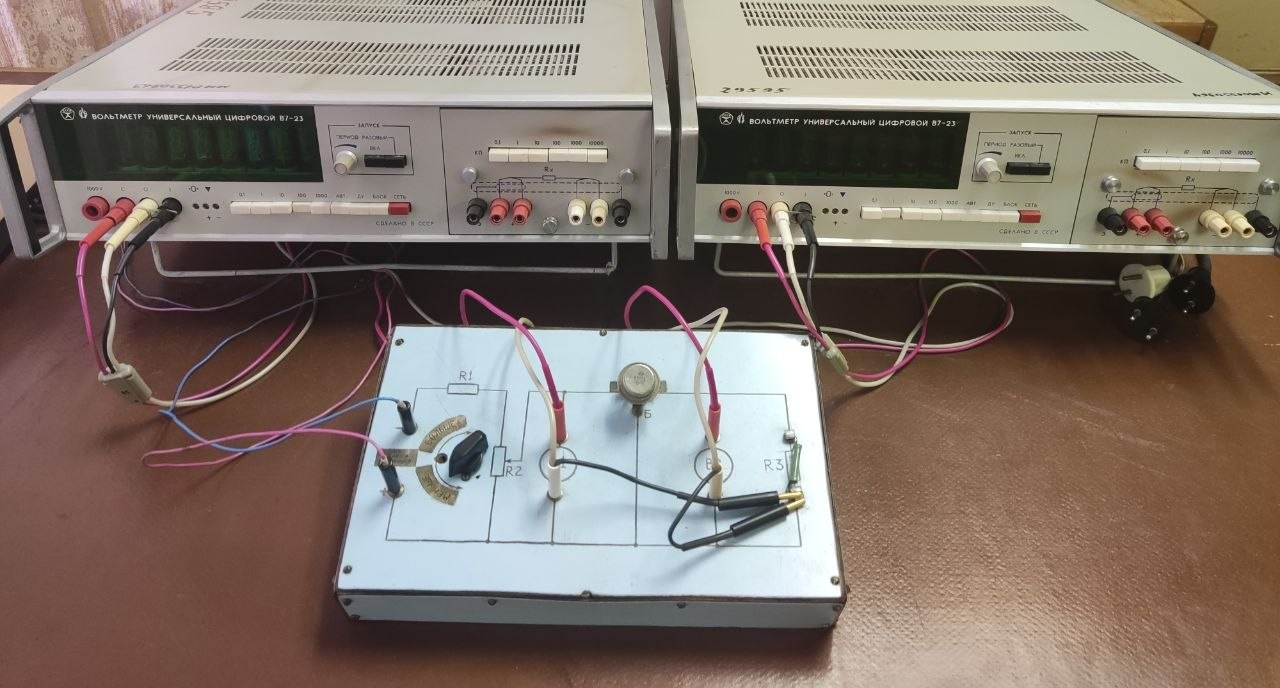
\includegraphics[width=\linewidth]{Device.jpg}
        \caption*{б) Фотография лабораторной установки}
    \end{minipage}
    \caption{Экспериментальная установка}
    \label{fig:setup}
\end{figure}

\subsection{Обработка данных и обсуждение результатов}
Измерения проводились при комнатной температуре $T = 298 \pm 0,5$ К. Исходные экспериментальные данные для грубой и точной шкал вольтметра V1 сведены в таблицы \ref{tab:raw1} и \ref{tab:raw2}.

\begin{table}[ht!]
\centering
\caption{Результаты измерений (Таблица 1, грубая шкала)}
\label{tab:raw1}
\small
\begin{tabular}{|c|c|c|c|c||c|c|c|c|c|}
\hline
№ & $U_{эб}$, В & $U_{кб}$, В & $I_k$, мА & $\ln I_k$ & № & $U_{эб}$, В & $U_{кб}$, В & $I_k$, мА & $\ln I_k$ \\ \hline
1 & 0.30 & 0.0019 & 0.158 & -1.843 & 9  & 0.38 & 0.0682 & 5.683 & 1.738 \\ \hline
2 & 0.31 & 0.0036 & 0.300 & -1.204 & 10 & 0.39 & 0.0848 & 7.067 & 1.955 \\ \hline
3 & 0.32 & 0.0053 & 0.442 & -0.817 & 11 & 0.40 & 0.1143 & 9.525 & 2.254 \\ \hline
4 & 0.33 & 0.0089 & 0.742 & -0.299 & 12 & 0.41 & 0.1380 & 11.500 & 2.442 \\ \hline
5 & 0.34 & 0.0156 & 1.300 & 0.262  & 13 & 0.42 & 0.1692 & 14.100 & 2.646 \\ \hline
6 & 0.35 & 0.0243 & 2.025 & 0.706  & 14 & 0.43 & 0.1968 & 16.400 & 2.797 \\ \hline
7 & 0.36 & 0.0352 & 2.933 & 1.076  & 15 & 0.44 & 0.2253 & 18.775 & 2.933 \\ \hline
8 & 0.37 & 0.0465 & 3.875 & 1.355  & 16 & 0.45 & 0.2502 & 20.850 & 3.037 \\ \hline
\end{tabular}
\end{table}

\begin{table}[ht!]
\centering
\caption{Результаты измерений (Таблица 1', точная шкала)}
\label{tab:raw2}
\small
\begin{tabular}{|c|c|c|c|c||c|c|c|c|c|}
\hline
№ & $U_{эб}$, В & $U_{кб}$, В & $I_k$, мА & $\ln I_k$ & № & $U_{эб}$, В & $U_{кб}$, В & $I_k$, мА & $\ln I_k$ \\ \hline
1 & 0.30 & 0.0016 & 0.133 & -2.015 & 9  & 0.38 & 0.0644 & 5.367 & 1.680 \\ \hline
2 & 0.31 & 0.0029 & 0.242 & -1.420 & 10 & 0.39 & 0.0853 & 7.108 & 1.961 \\ \hline
3 & 0.32 & 0.0052 & 0.433 & -0.836 & 11 & 0.40 & 0.1082 & 9.017 & 2.199 \\ \hline
4 & 0.33 & 0.0089 & 0.742 & -0.299 & 12 & 0.41 & 0.1326 & 11.050 & 2.402 \\ \hline
5 & 0.34 & 0.0142 & 1.183 & 0.168  & 13 & 0.42 & 0.1684 & 14.033 & 2.641 \\ \hline
6 & 0.35 & 0.0221 & 1.842 & 0.611  & 14 & 0.43 & 0.1963 & 16.358 & 2.795 \\ \hline
7 & 0.36 & 0.0333 & 2.775 & 1.021  & 15 & 0.44 & 0.2219 & 18.492 & 2.917 \\ \hline
8 & 0.37 & 0.0501 & 4.175 & 1.429  & 16 & 0.45 & 0.2464 & 20.533 & 3.022 \\ \hline
\end{tabular}
\end{table}

Обработка результатов производилась с помощью скрипта на языке Python с использованием самостоятельно реализованной универсальной функции для метода парных точек. Результаты расчета параметров прямых сведены в таблицы \ref{tab:paired1} и \ref{tab:paired2}.

\begin{table}[ht!]
\centering
\caption{Расчет методом парных точек (Таблица 2, грубая шкала)}
\label{tab:paired1}
\footnotesize
\begin{tabular}{|c|c|c|c|c|c|c|c|c|c|}
\hline
№ & $x_{II}$ & $x_I$ & $\Delta x$ & $y_{II}$ & $y_I$ & $\Delta y$ & $a_i$ & $a_i - \bar{a}$ & $(a_i - \bar{a})^2$ \\ \hline
1 & 0.38 & 0.30 & 0.08 & 1.738 & -1.843 & 3.581 & 44.76 & 12.63 & 159.5 \\ \hline
2 & 0.39 & 0.31 & 0.08 & 1.955 & -1.204 & 3.159 & 39.49 & 7.36 & 54.2 \\ \hline
3 & 0.40 & 0.32 & 0.08 & 2.254 & -0.817 & 3.071 & 38.39 & 6.26 & 39.2 \\ \hline
4 & 0.41 & 0.33 & 0.08 & 2.442 & -0.299 & 2.741 & 34.26 & 2.13 & 4.5 \\ \hline
5 & 0.42 & 0.34 & 0.08 & 2.646 & 0.262 & 2.384 & 29.80 & -2.33 & 5.4 \\ \hline
6 & 0.43 & 0.35 & 0.08 & 2.797 & 0.706 & 2.091 & 26.14 & -5.99 & 35.9 \\ \hline
7 & 0.44 & 0.36 & 0.08 & 2.933 & 1.076 & 1.857 & 23.21 & -8.92 & 79.6 \\ \hline
8 & 0.45 & 0.37 & 0.08 & 3.037 & 1.355 & 1.682 & 21.03 & -11.10 & 123.2 \\ \hline
\multicolumn{7}{|r|}{Сумма:} & 257.08 & & 501.5 \\ \hline
\end{tabular}
\end{table}

\begin{table}[ht!]
\centering
\caption{Расчет методом парных точек (Таблица 2', точная шкала)}
\label{tab:paired2}
\footnotesize
\begin{tabular}{|c|c|c|c|c|c|c|c|c|c|}
\hline
№ & $x_{II}$ & $x_I$ & $\Delta x$ & $y_{II}$ & $y_I$ & $\Delta y$ & $a_i$ & $a_i - \bar{a}$ & $(a_i - \bar{a})^2$ \\ \hline
1 & 0.38 & 0.30 & 0.08 & 1.680 & -2.015 & 3.695 & 46.19 & 13.44 & 180.6 \\ \hline
2 & 0.39 & 0.31 & 0.08 & 1.961 & -1.420 & 3.381 & 42.26 & 9.51 & 90.4 \\ \hline
3 & 0.40 & 0.32 & 0.08 & 2.199 & -0.836 & 3.035 & 37.94 & 5.19 & 26.9 \\ \hline
4 & 0.41 & 0.33 & 0.08 & 2.402 & -0.299 & 2.701 & 33.76 & 1.01 & 1.0 \\ \hline
5 & 0.42 & 0.34 & 0.08 & 2.641 & 0.168 & 2.473 & 30.91 & -1.84 & 3.4 \\ \hline
6 & 0.43 & 0.35 & 0.08 & 2.795 & 0.611 & 2.184 & 27.30 & -5.45 & 29.7 \\ \hline
7 & 0.44 & 0.36 & 0.08 & 2.917 & 1.021 & 1.896 & 23.70 & -9.05 & 81.9 \\ \hline
8 & 0.45 & 0.37 & 0.08 & 3.022 & 1.429 & 1.593 & 19.91 & -12.84 & 164.9 \\ \hline
\multicolumn{7}{|r|}{Сумма:} & 262.00 & & 578.8 \\ \hline
\end{tabular}
\end{table}

\textbf{Результаты аппроксимации (доверительный интервал 95\%, $t = 2.365$):}
\begin{itemize}
    \item Выборка 1 (грубая): $a = 32.14 \pm 7.08$ В$^{-1}$, $b = -10.86 \pm 2.65$.
    \item Выборка 2 (точная): $a = 32.75 \pm 7.60$ В$^{-1}$, $b = -11.14 \pm 2.85$.
\end{itemize}

Графики экспериментальных точек и аппроксимирующих кривых (экспоненциальные и логарифмические) представлены на рисунках 2 и 3.

\begin{figure}[ht!]
    \centering
    \begin{minipage}{0.48\textwidth}
        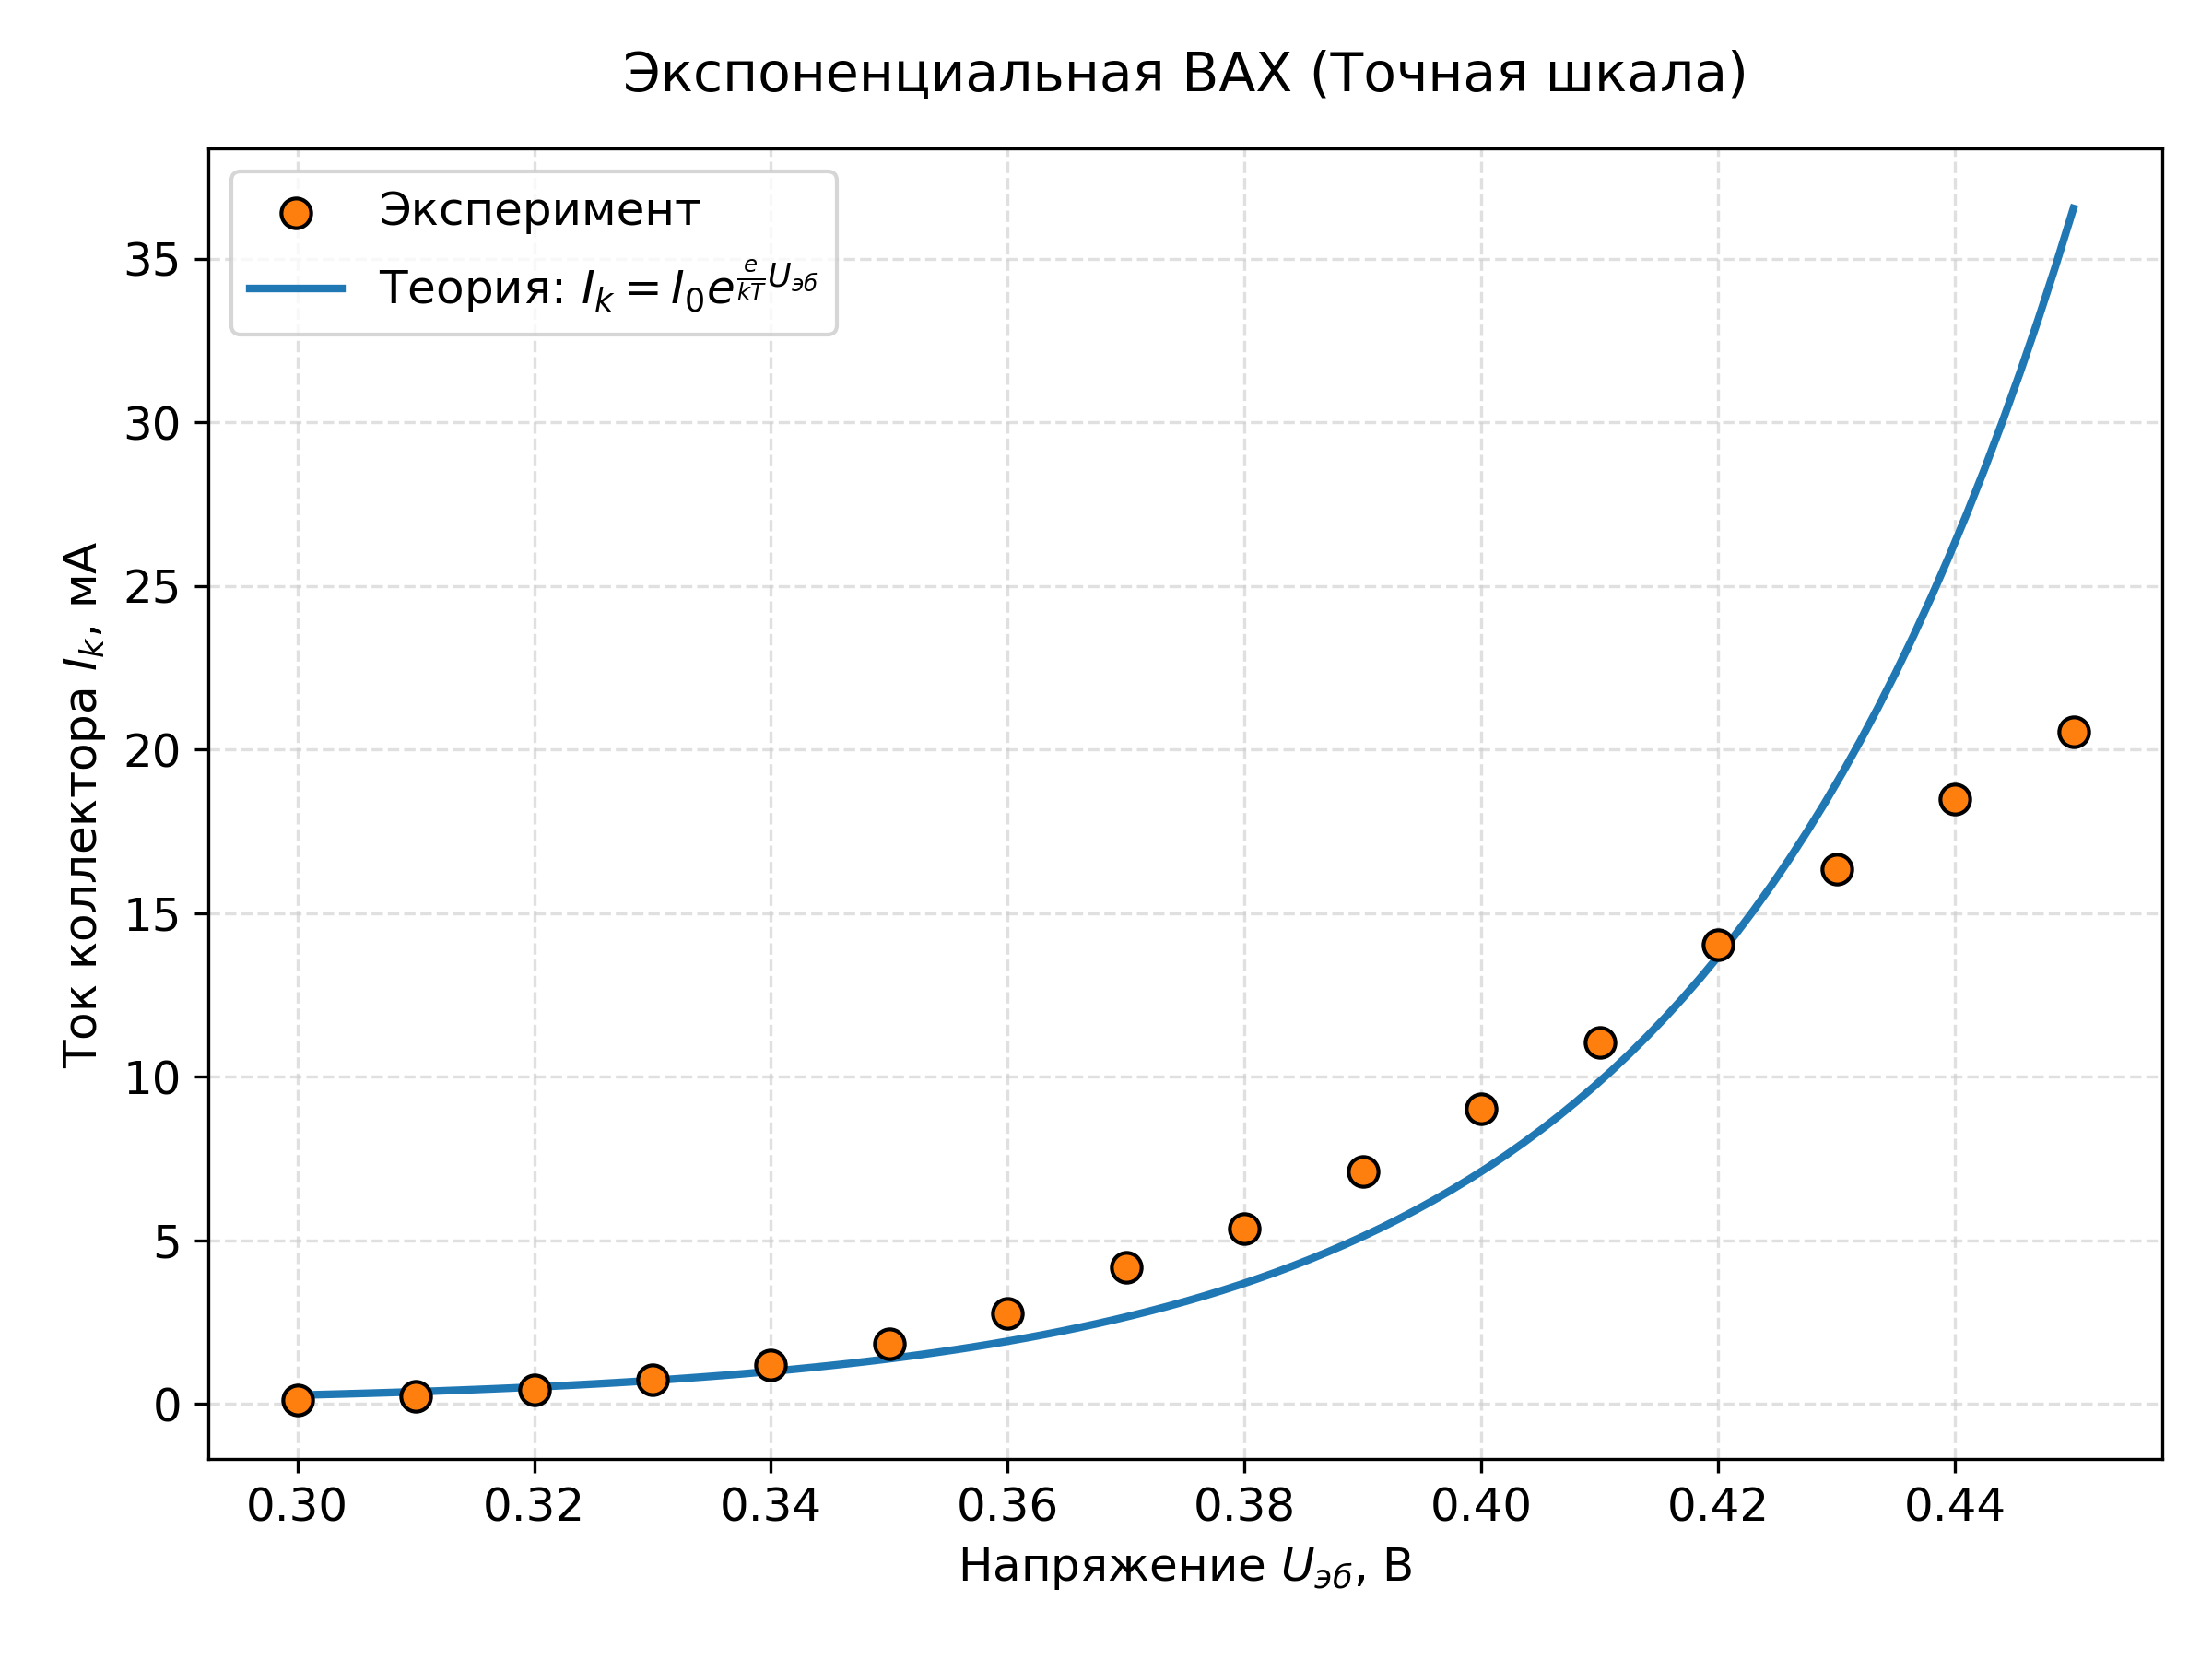
\includegraphics[width=\linewidth]{exp_plot_fine.png}
    \end{minipage}
    \hfill
    \begin{minipage}{0.48\textwidth}
        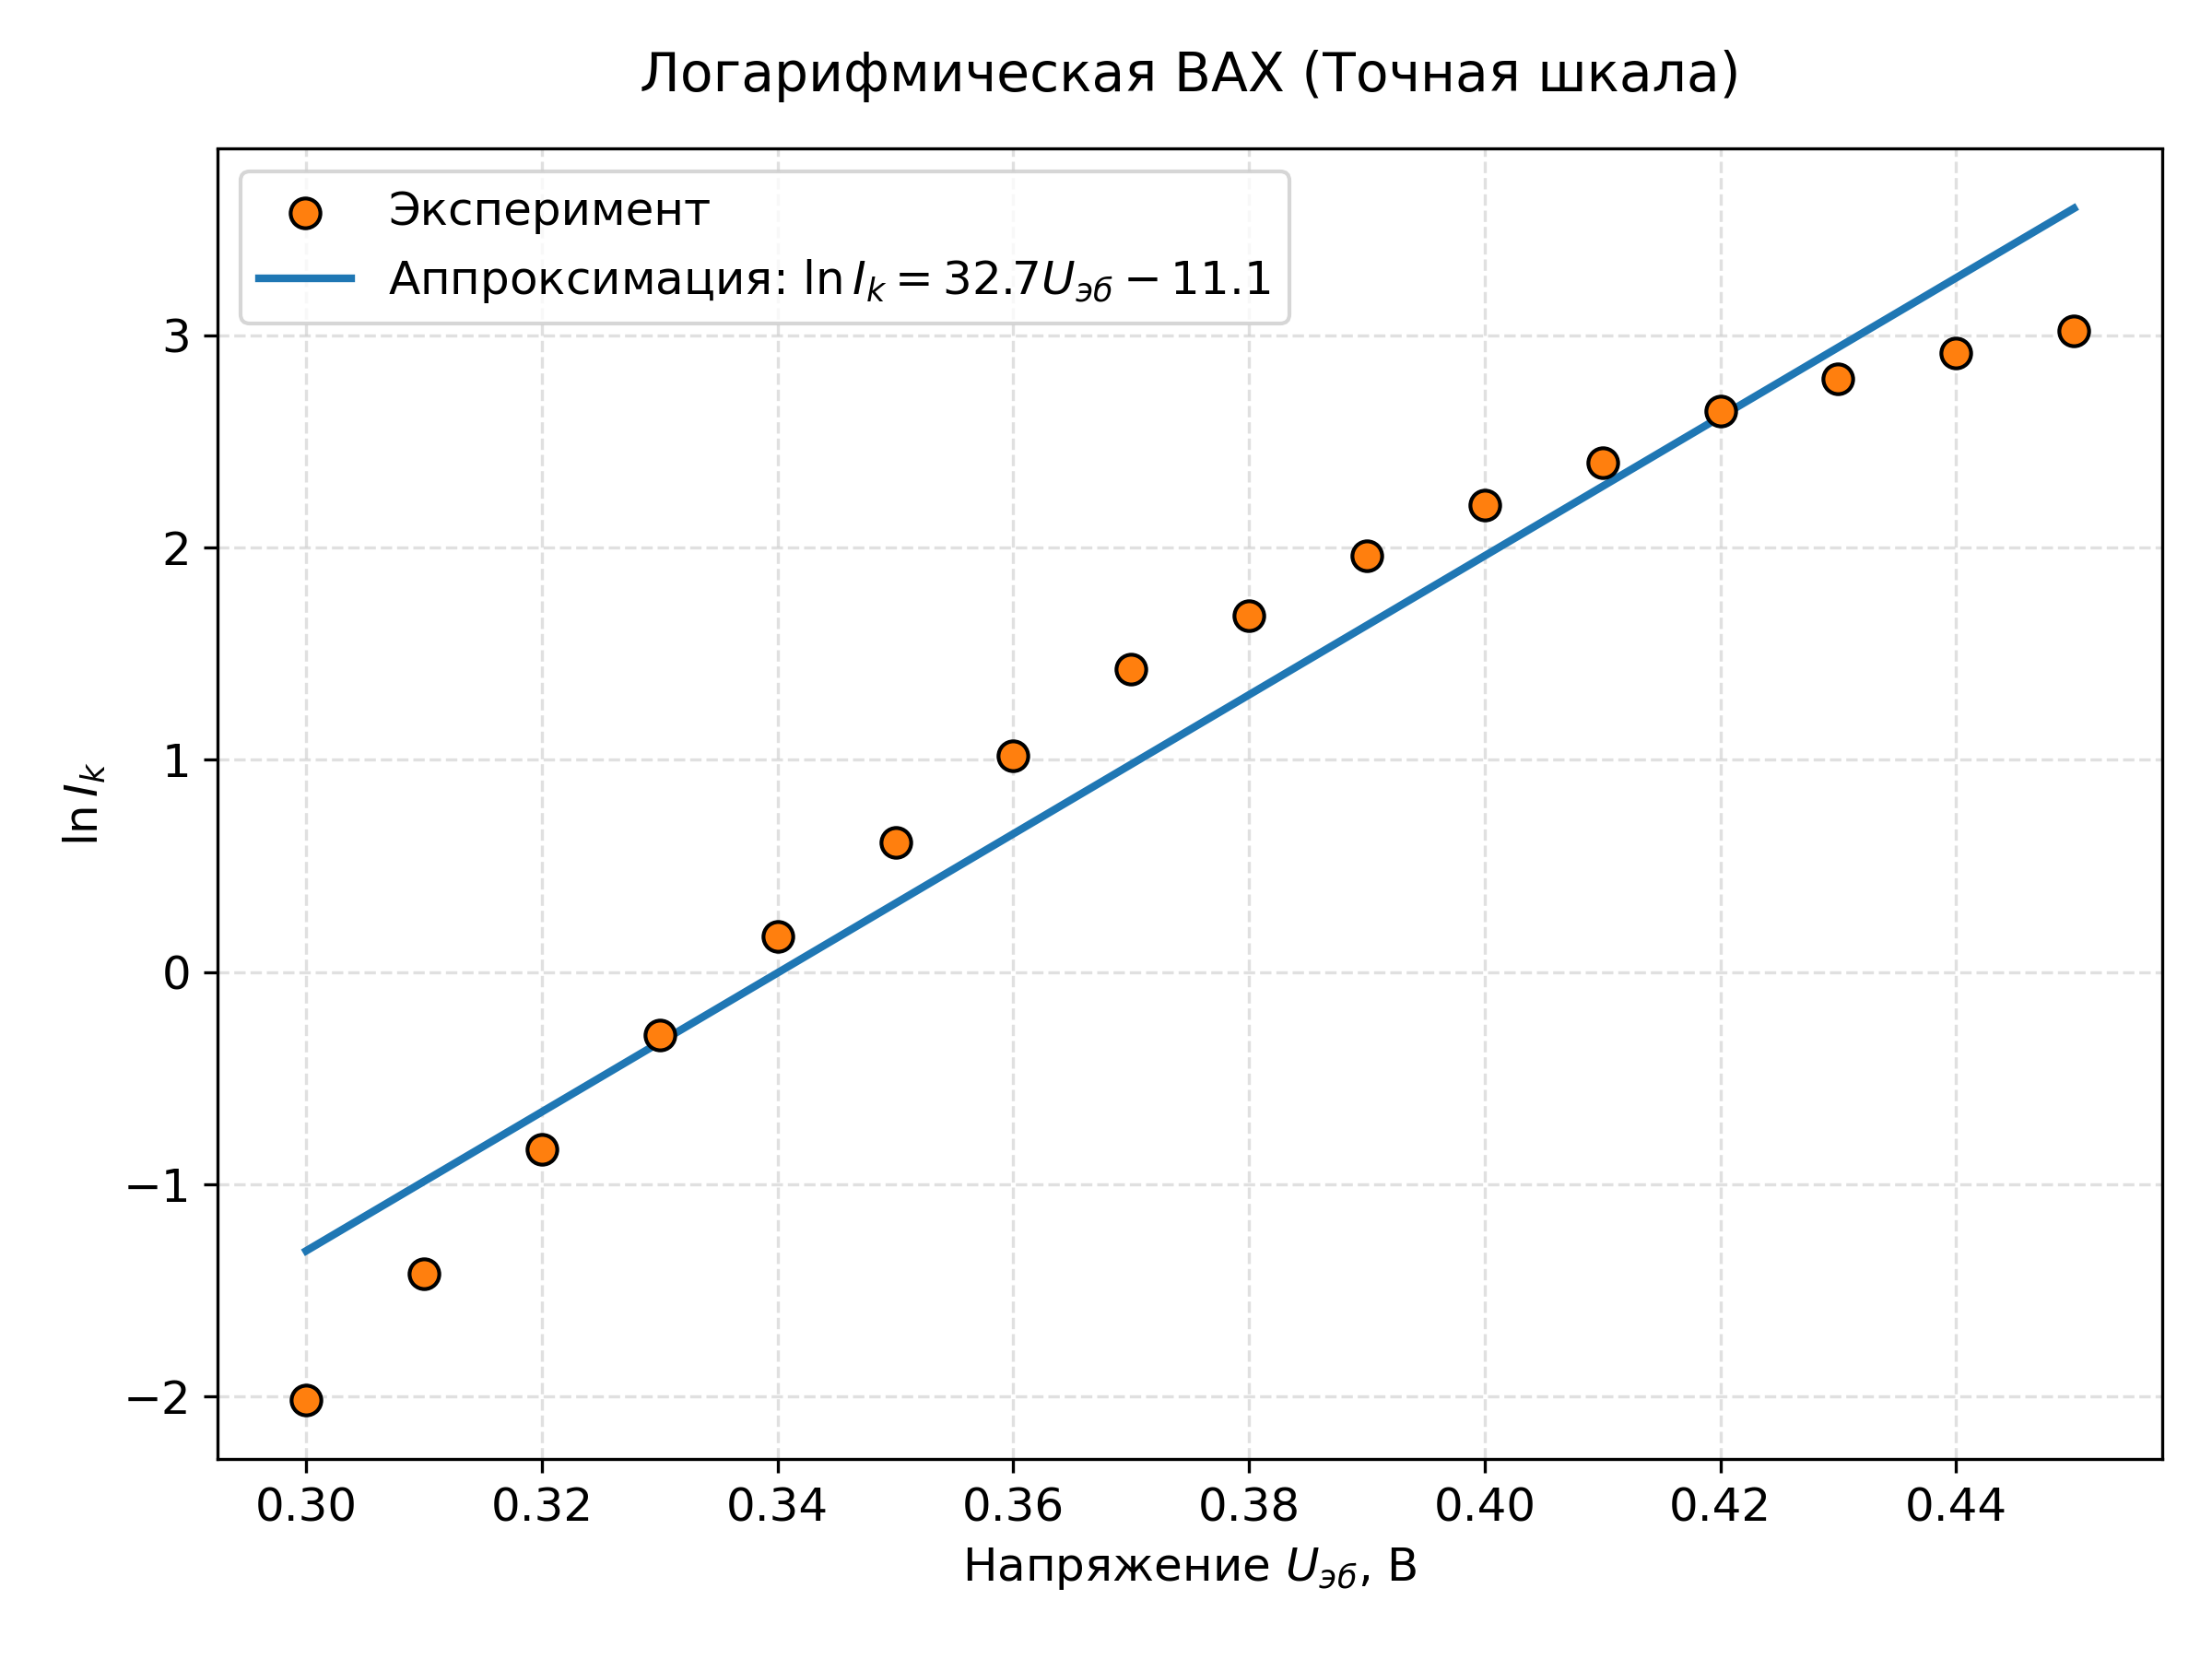
\includegraphics[width=\linewidth]{log_plot_fine.png}
    \end{minipage}
    \caption{Экспоненциальная и логарифмическая ВАХ (Точная шкала)}
\end{figure}

\begin{figure}[ht!]
    \centering
    \begin{minipage}{0.48\textwidth}
        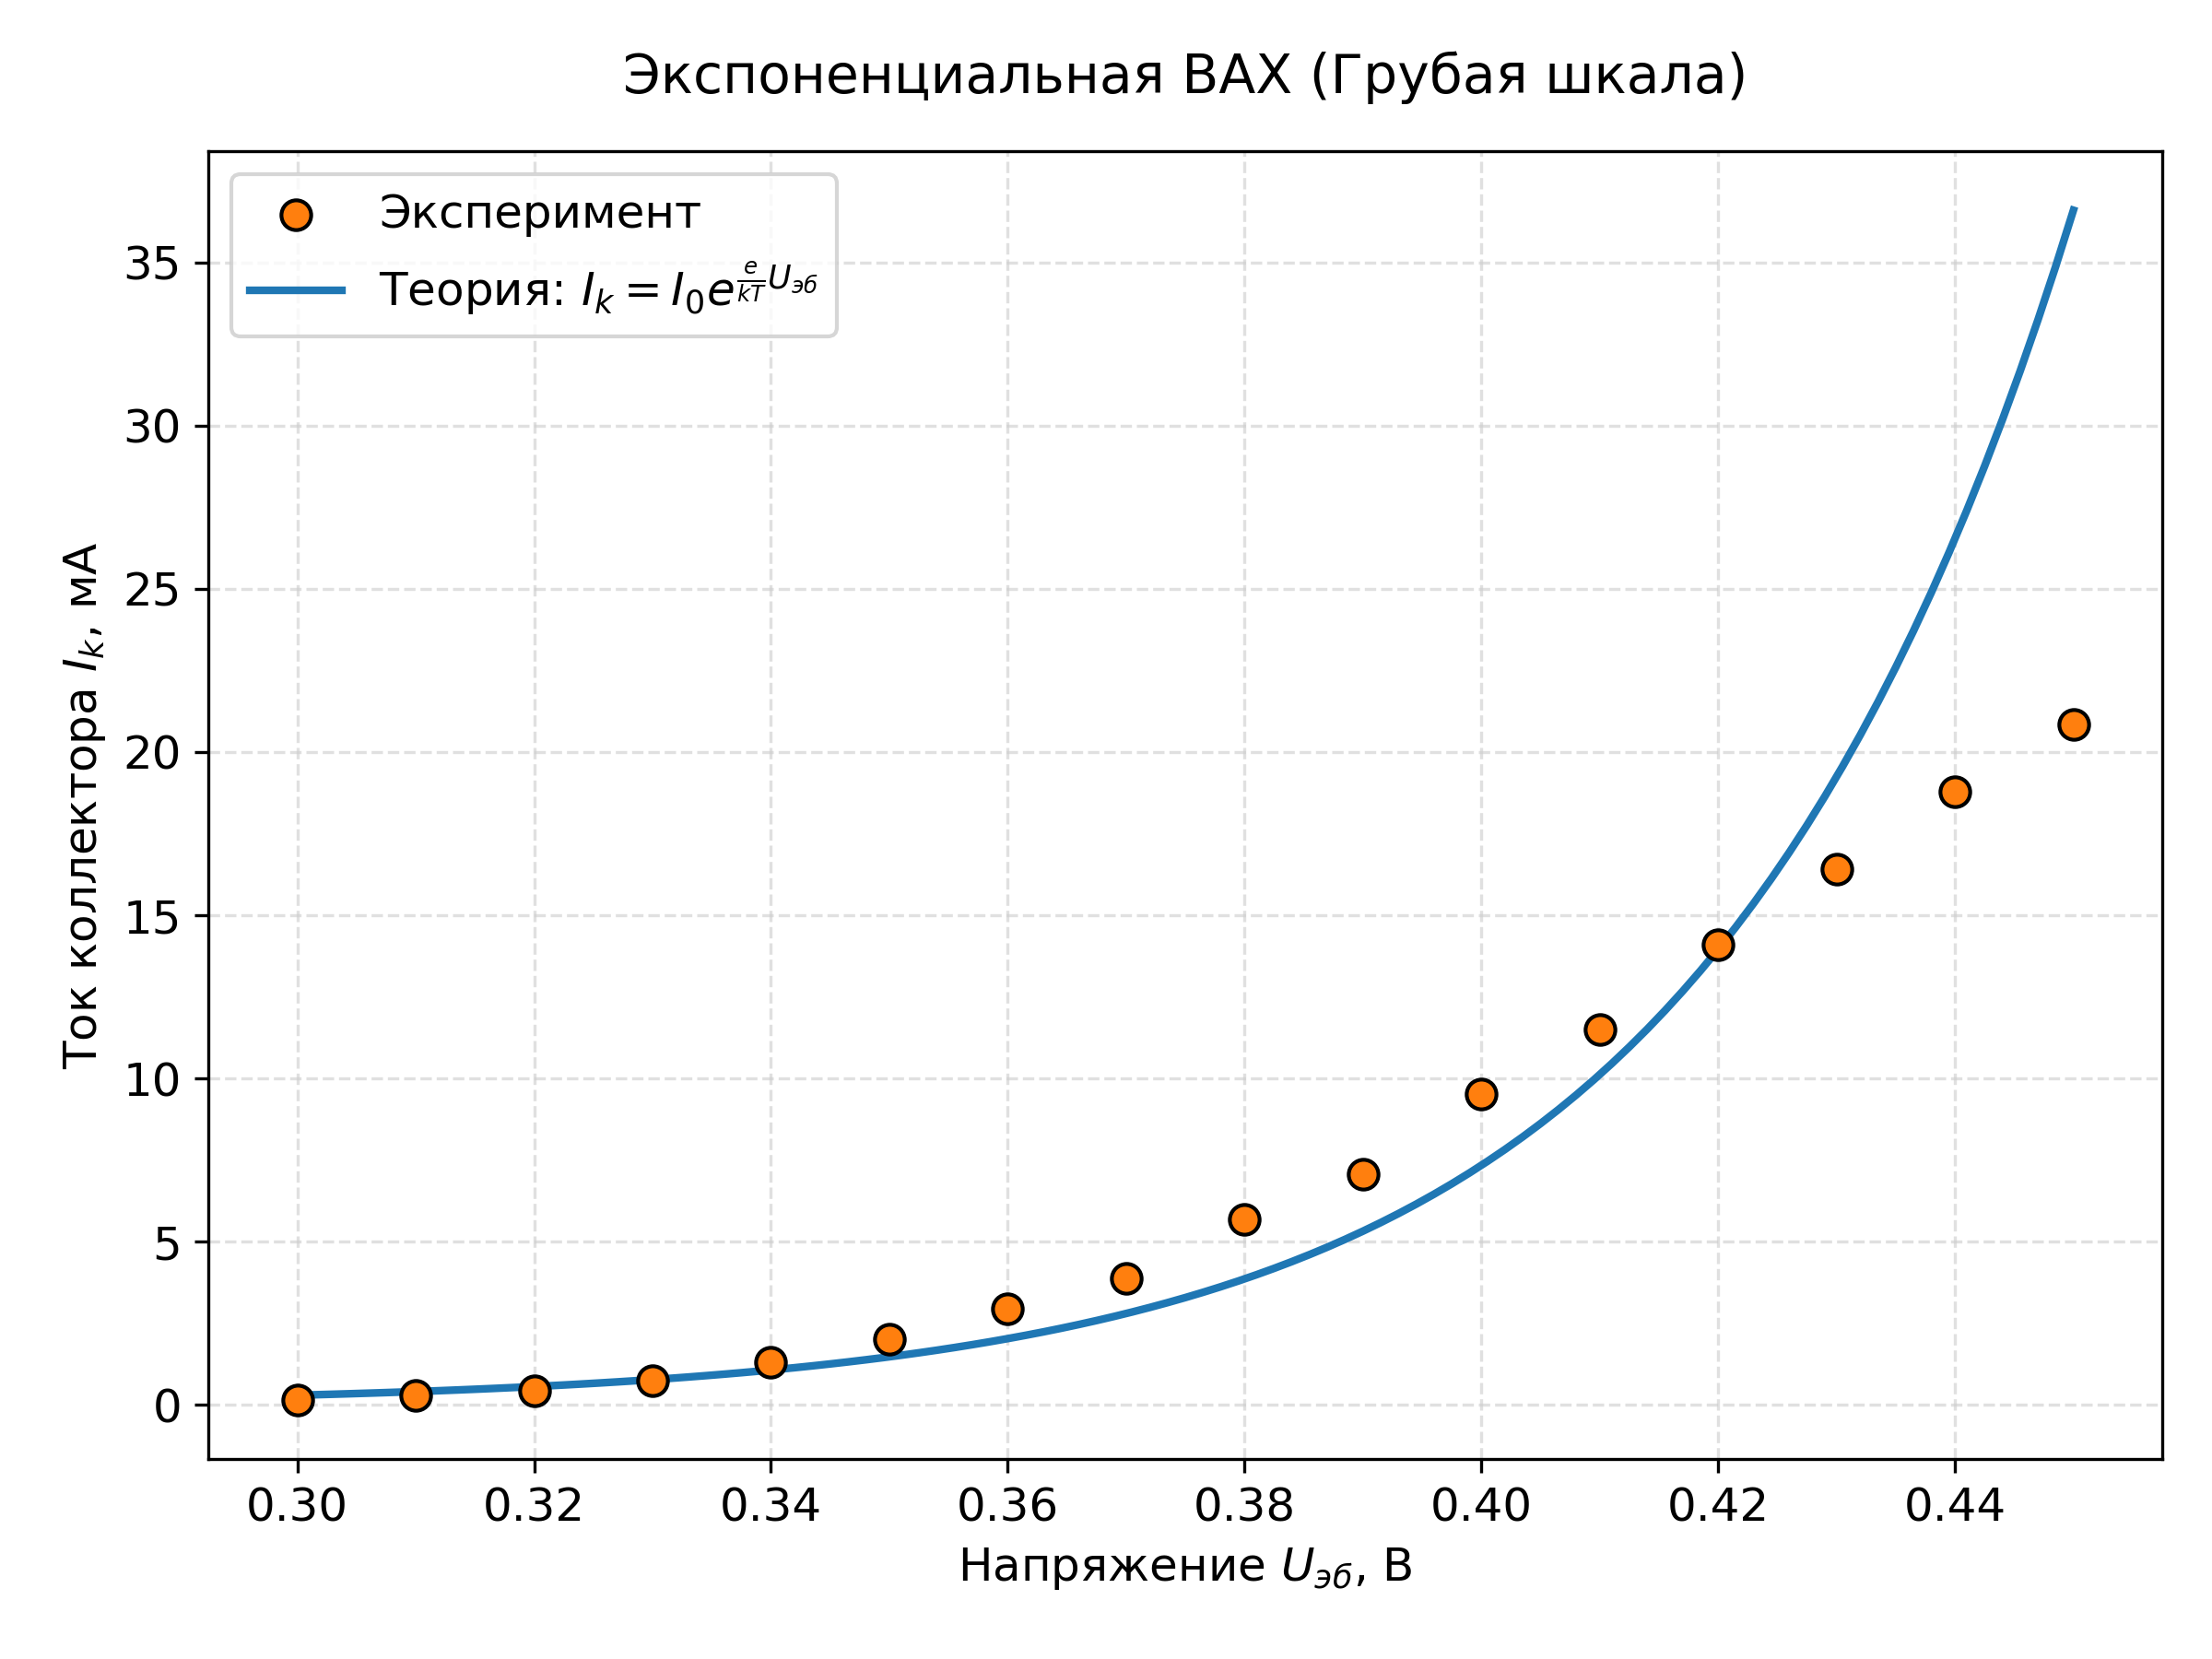
\includegraphics[width=\linewidth]{exp_plot_coarse.png}
    \end{minipage}
    \hfill
    \begin{minipage}{0.48\textwidth}
        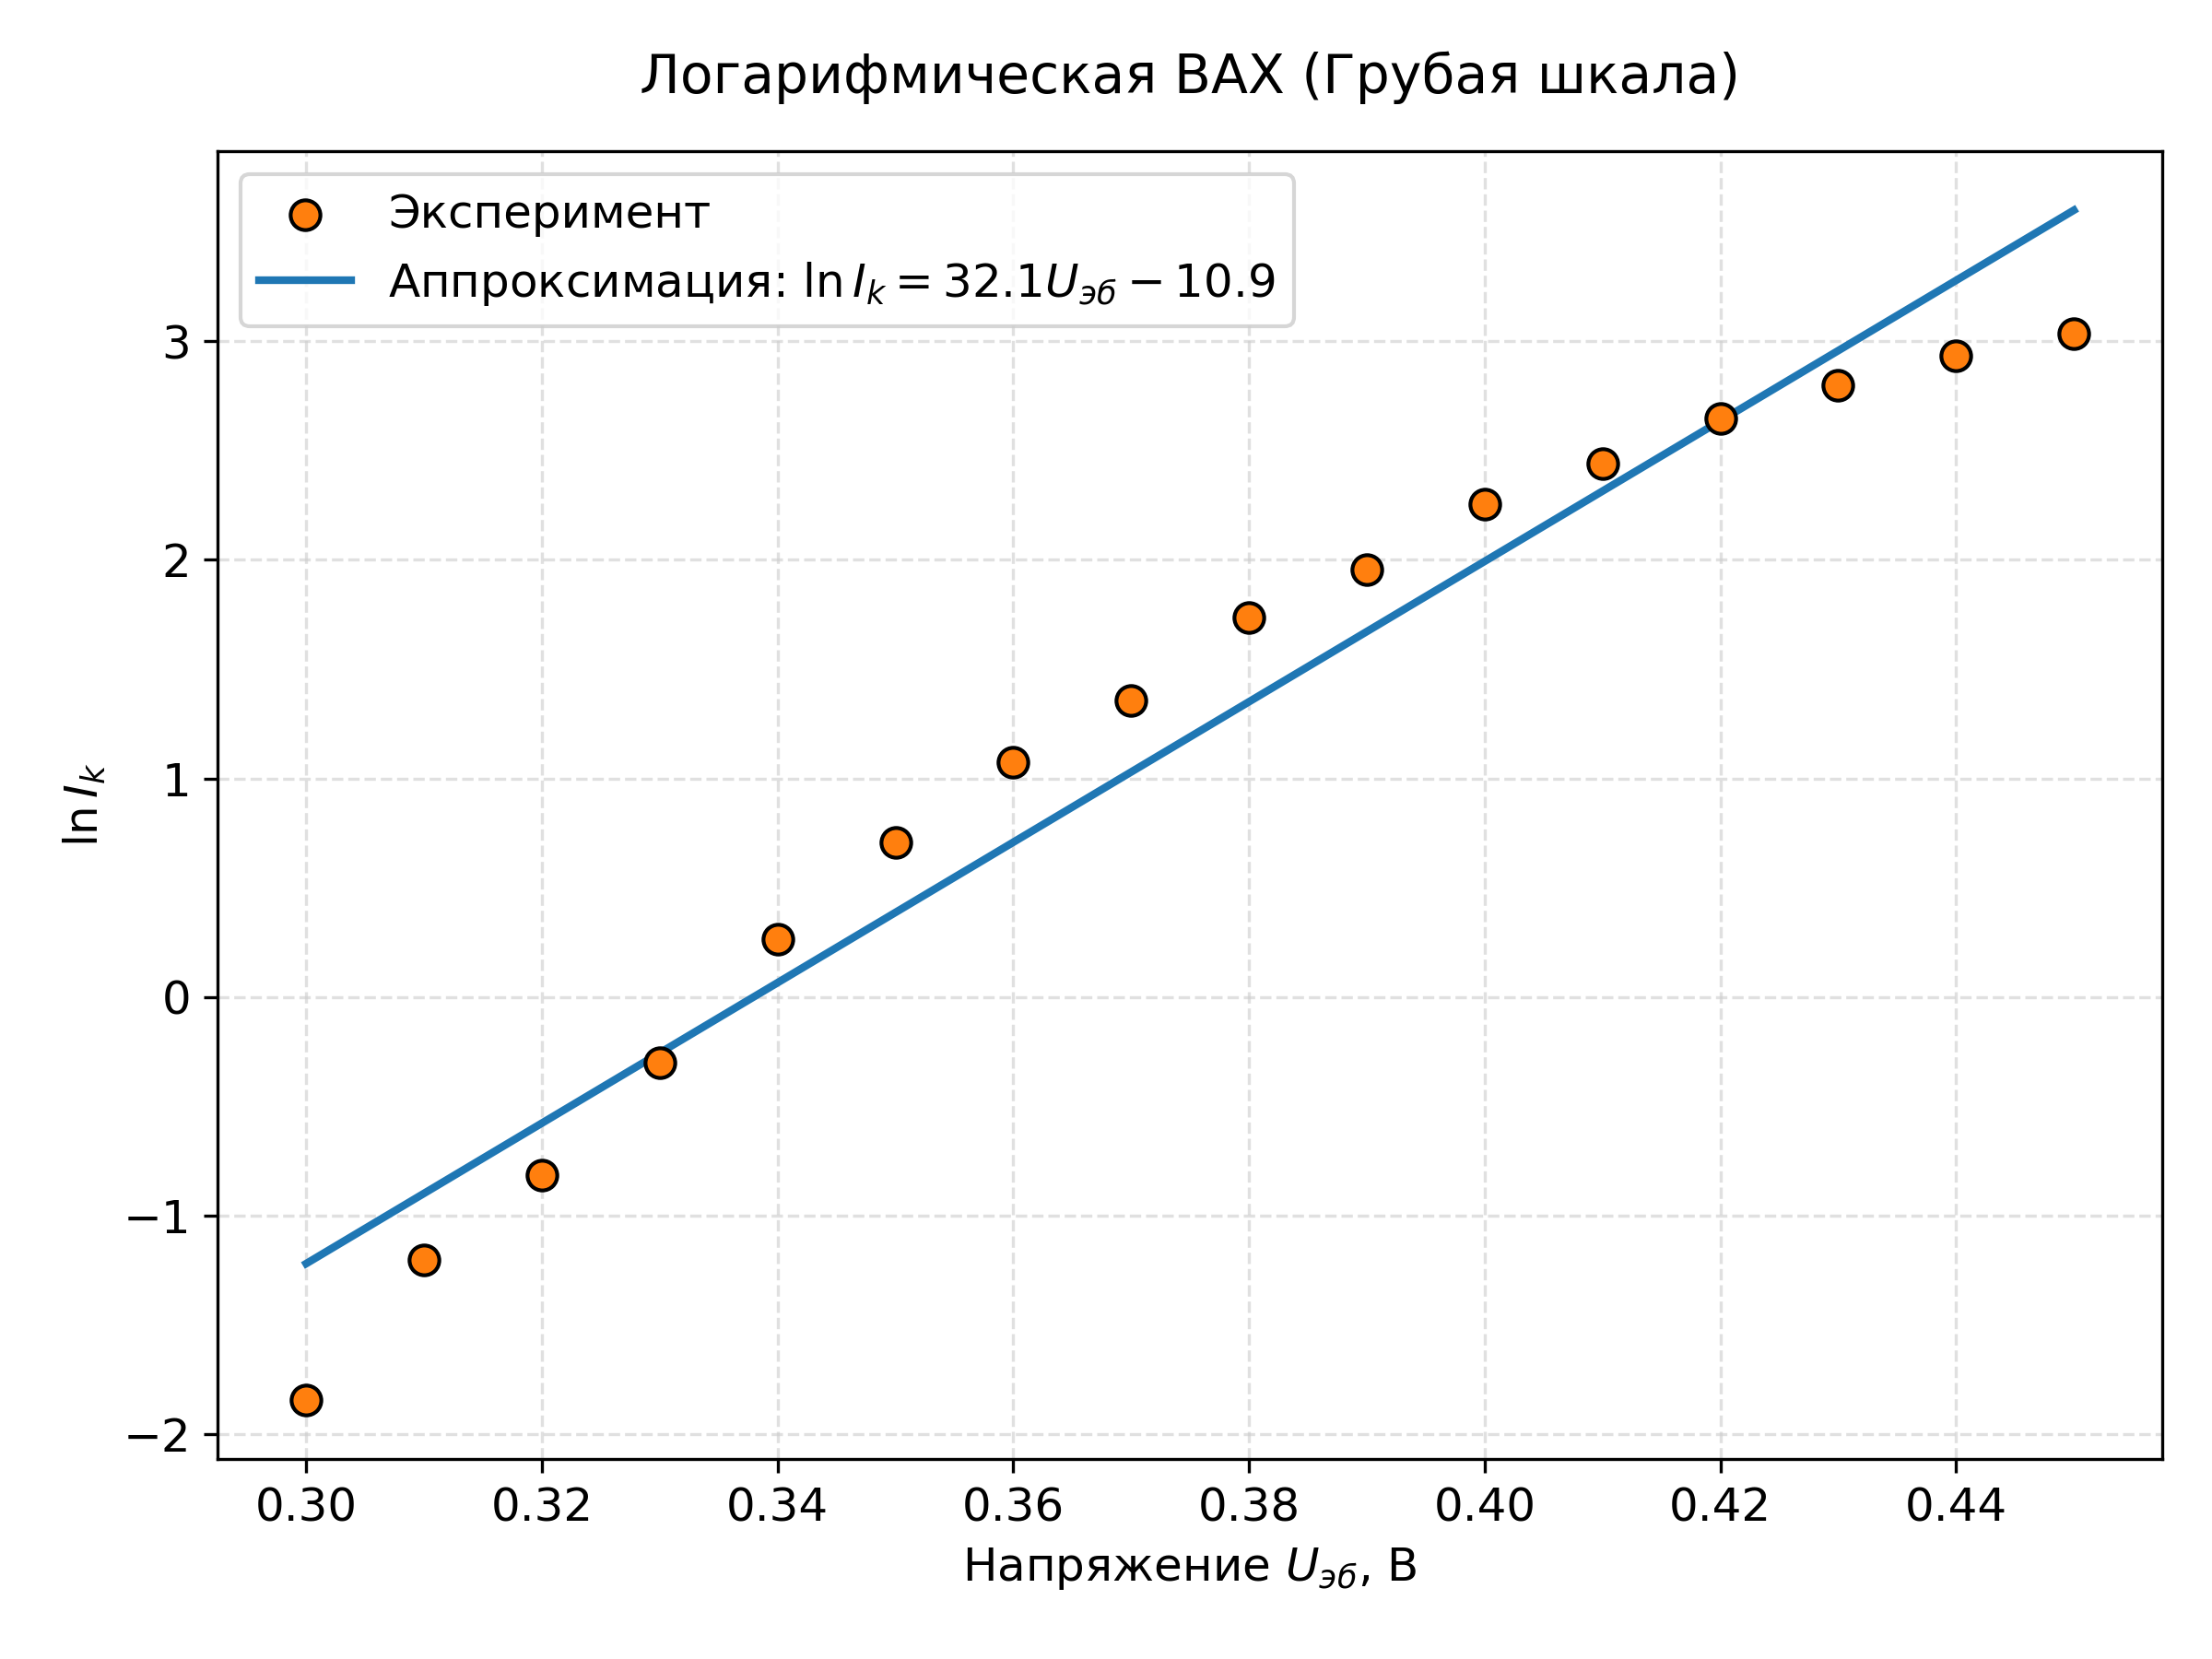
\includegraphics[width=\linewidth]{log_plot_coarse.png}
    \end{minipage}
    \caption{Экспоненциальная и логарифмическая ВАХ (Грубая шкала)}
\end{figure}

\textbf{Расчет отношения $e/k$:} \\
Теоретическое значение: $(e/k)_{теор} = \frac{1.602 \cdot 10^{-19}}{1.38 \cdot 10^{-23}} \approx 11604$ К/В.

Экспериментальные значения:
\begin{itemize}
    \item Выборка 1: $e/k = 32.136 \cdot 298 = 9577 \pm 2109$ К/В.
    \item Выборка 2: $e/k = 32.750 \cdot 298 = 9759 \pm 2266$ К/В.
\end{itemize}

\section{Выводы}
В ходе лабораторной работы была успешно измерена вольт-амперная характеристика эмиттерного перехода биполярного транзистора. Использование математического метода парных точек (реализованного в виде единой универсальной функции на Python) позволило объективно провести линейную аппроксимацию данных и вычислить константу $e/k \approx 9759 \pm 2266$ К/В (для точной шкалы вольтметра). 

Полученное экспериментальное значение несколько ниже идеального теоретического ($11604$ К/В). Это полностью согласуется с физикой реальных полупроводниковых приборов: в реальном p-n переходе диффузионный ток описывается уравнением с учетом \textbf{коэффициента неидеальности} $\eta$ ($I_k \sim e^{\frac{e}{\eta kT}U_{эб}}$), который учитывает токи рекомбинации в обедненной области. Отношение теоретического значения к экспериментальному дает $\eta = 11604 / 9759 \approx 1.18$, что является отличным показателем для кремниевых транзисторов (где $\eta$ обычно лежит в пределах от 1 до 2). 

Сравнение двух выборок показало, что использование точной шкалы (Выборка 2) позволило минимизировать приборную погрешность на малых напряжениях, что сделало логарифмическую кривую визуально более сглаженной. Относительно высокая погрешность итогового результата ($\approx 23\%$) связана с тем, что метод парных точек крайне чувствителен к микроскопическим отклонениям графика от строгой линейности на краях диапазона измерения. В целом, математическая модель биполярного транзистора полностью подтвердилась экспериментально.